\documentclass[12pt]{book}


\usepackage[utf8]{inputenc}
\usepackage[T1]{fontenc}
\usepackage{geometry}
\usepackage{graphicx}
\usepackage[spanish]{babel}
\usepackage{amsthm}
\usepackage{amsmath}
\usepackage{calrsfs}
\usepackage{trfsigns}

\newtheorem{thm}{Teorema}[section]
\theoremstyle{definition}
\newtheorem{dfn}{Definición}[section]
\theoremstyle{remark}
\newtheorem{note}{Nota}[section]
\theoremstyle{plain}
\newtheorem{lem}[thm]{Lema}

\geometry{letterpaper}



\title{Celdas de Combustible}
\author{Dr. Casimiro Gómez González\\
	Facultad de Electrónica, UPAEP\\
               correo: casimiro.gomez@upaep.mx\\
               Tel: 222 229 9428}
\date{Primavera 2010}

\begin{document}
\frontmatter
\maketitle


\chapter{Prólogo}

El presente material es producto del estudio realizado para diseñar celdas de combustible

\begin{flushright}

El autor\\
Casimiro Gómez González\\
Doctor en Ingeniería Mecatrónica
\end{flushright}

\tableofcontents

\mainmatter
\chapter{Introducción}
Una celda de combustible consiste de un electrodo cargado negativamente (ánodo), un electrodo cargado positivamente (cátodo), y un electrolito de membrana. El hidrógeno es oxidado en el ánodo y el oxigeno es reducido en el cátodo. 
Los protones son transportados desde el ánodo a el cátodo a través del electrolito de membrana, y los electrones son transportados a el cátodo  a través del circuito externo. 
En la naturaleza, las moléculas no pueden estar en estado iónico, por lo tanto se recombinan inmediatamente con otras moléculas para regresar a su estado neutral. 
Los protones de hidrógeno en las celdas de combustible permanecen en estado iónico viajando de molécula a molécula a través del uso de materiales especiales. Los protones 
viajan a través de la membrana de polímero hecha de ácido persulfunato con una estructura de Teflón.  Los electrones son atraídos a el material conductor y viajan a el carga 
cuando se necesita. En el cátodo, el oxigeno reacciona con protones y electrones, formando agua y produciendo calor. Tanto  el ánodo y como el cátodo contiene un catalizador
 para incrementar la velocidad del proceso electroquímico, como se muestra en la figura \ref{fig1}.

\begin{figure}
\centering
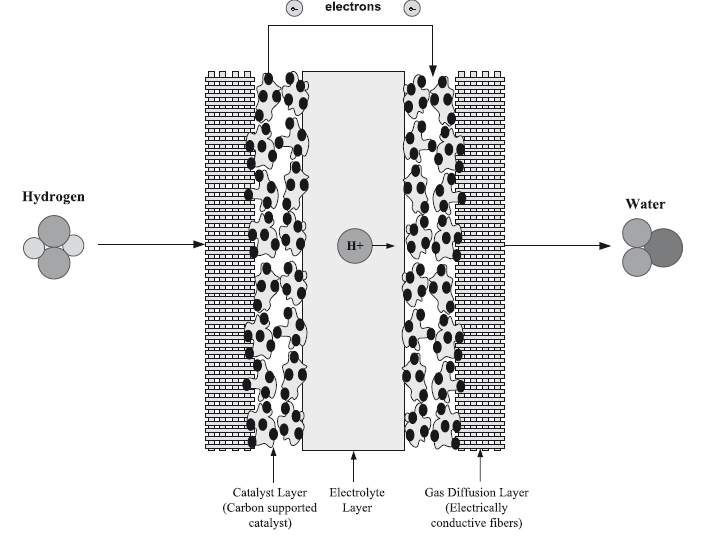
\includegraphics[width=4in]{Celdasdecombustible.png}
\caption{Configuración de una simple  Celda de combustible}
\label{fig1}
\end{figure}

Una celda de combustible típica (celda de combustible con membrana de intercambio protónico) tiene las siguientes reacciones:


\begin{align*}
Anodo: & H_2 (g) \rightarrow 2 H^{+}(aq)+2 e^{-} \\
Catodo: & \frac{1}{2} O_2 (g) + 2 H^{+}(aq)+2 e^{-} \rightarrow H_{2} O (l) \\
Total: & H_2(g) + \frac{1}{2} O_2 (g) \rightarrow H_{2}O (l)+ Energía Eléctrica+calor
\end{align*}


Los reactantes son transportados por difusión y/o convección a la superficie  catalizada del electrodo donde las reacciones electroquímicas se realizan. El agua y el calor 
generados por la celda de combustible deben ser continuamente removidos y pueden se un tema muy importante en el comportamiento de la celda de combustible.

La pila básica de celdas de combustible PEM consiste de una membrana de intercambio protónico (PEM), capas de  catalizador y  capas de difusores de gas, placas de flujo de 
campo, juntas y placas de extremo. Esta compuesta de los siguientes elementos:

\begin{itemize}
\item \textbf{Membrana de Intercambio Protónico}.- La cual permite que los protones de Hidrógeno viajen del ánodo al cátodo y esta compuesta por una Membrana ácida de Persulfatos (nafion 112, 115, 117).
\item \textbf{Capas de catalizador}.- Rompe el combustible en protones y electrones. Los protones se combinan con el oxidante para formar agua en el cátodo de la celda de combustible. Los electrones viajan a la carga. Los catalizadores son de Platino/carbón.
\item \textbf{Capas del difusor de gas}.- Permite el combustible/oxidante viajar a través de las capas porosas, mientras se colectan electrones. Esta formado por paños de carbón o papel Toray.
\item \textbf{Placas de flujo de campo}.- distribuye el combustible y el oxidante a la capa de difusión de gas. Esta hecho de grafito, o de acero inoxidable.
\item \textbf{Juntas}.- Evitar fugas de combustible y ayuda a distribuir la presión uniformemente. Esta hecha de silicón, o Teflón.
\item \textbf{Placas de terminación}.- Mantiene las capas de la pila en su lugar. Están hechas de acero inoxidable, grafito, polietileno, y PVC.
\end{itemize}

Algunas ventajas de los sistemas de celdas de combustible son las siguientes:

\begin{itemize}
\item Las celdas de combustible tienen el potencial de operar con una alta eficiencia
\item Hay muchos tipos de fuentes de combustible y métodos para suministrar combustible a la celda de combustible.
\item Las celdas de combustible tienen un diseño altamente escalable.
\item Las celdas de combustible no producen contaminación
\item Las celdas de combustible tiene un mantenimiento bajo porque no tiene partes móviles
\item Las celdas de combustible no necesitan ser recargables, y proporcionan energía instantáneamente cuando se proporciona el combustible.
\end{itemize}

\section{Breve descripción histórica}

A William Grove se le reconoce el invento de la primera celda de combustible en 1839. Las celdas de combustible no fueron muy investigadas durante los 1800 y principios de 
los 1900s. 
Las investigaciones exhaustivas comenzaron durante 1960 en la NASA. 
Durante la última década, las celdas de combustible han sido investigadas exhaustivamente y están cada vez más cerca de la comercialización. 
A continuación se presenta un breve resumen histórico.

\begin{itemize}
 \item En 1800, W. Nicholson y A. Carlisle describieron el proceso de utilizar la electricidad para romper las moléculas del agua
 \item En  1836, William Grove demuestra el funcionamiento de una celda de combustible
 \item En 1889, Equipos separados: L. Mond y C. Langer/ C. Wright y C. Thompson/L. Cailleteton y L. Colardeau realizaron varios experimentos con celdas de combustible.
 \item En 1893, F. Ostwald describe las funciones de los componentes de las celdas de combustible.
 \item En 1896, W. Jacques construye una batería de carbon.
 \item A principios de 1900, E. Baur y sus estudiantes realizaron experimentos con dispositivos a altas temperaturas.
 \item En 1960, T. Grubb y L. Niedrach inventaron la tecnología PEMFC en General Electric.
 \item Desde 1990 hasta el presente, las investigaciones de celdas de combustible han sido intensivas en todos los tipos de celdas de combustible.
\end{itemize}

El proceso de utilizar electricidad para romper las moléculas de agua en hidrógeno y oxigeno
(electrólisis) fue descrito por primera vez en 1800 por William Nicholson y Anthony Carlisle. William
Grove inventó la primera celda de combustible en 1839, usando la idea de Nicholson y Carlisle
para ``recomponer agua''. El realizó esto combinando electrodos en un circuito en serie,
con electrodos de platino separados en oxigeno e hidrógeno, sumergidos en un electrolito que es 
una solución de ácido sulfúrico diluido. La batería de gas, o Celda Grove, generaba 12 amp de
corriente y cerca de 1,8 volts.
La NASA investigo la tecnología de celdas de combustible tipo PEM para el proyecto Gemini a inicios
del programa espacial de los Estados Unidos. Las baterías fueron usadas para los proyectos
anteriores de las misiones Mercurio, pero el proyecto Apolo necesitaba una fuente de poder
mayor y que durara un periodo de tiempo mayor. Desafortunadamente, las primeras celda de combustible
tipo PEM tenian dificultades con la contaminación interna y el filtrado de oxigeno a 
a través de la membrana. General Electric rediseño su celda de combustible, y el nuevo
modelo se comporto adecuadamente por el resto de los vuelos de el Gemini. Los diseñadores 
del proyecto Apolo y los transbordadores espaciales últimamente han escogido las celdas 
de combustible alcalinas.

General Electric continuo trabajando en celdas de combustible tipo PEM en los 70s, y diseño
la tecnología de electrolisis por PEM, la cual proporcionó a la naval de US plantas 
generadoras de oxigeno. La real naval Británica uso celdas de combustible PEM a principios
de los 80s para su flota submarina y durante la década pasada, las celdas de combustible 
tipo PEM han sido investigadas extensivamente por compañías comerciales para transporte, 
aplicaciones estacionarias y aplicaciones de potencia portátiles.


\section{Modelos matemáticos}

Los modelos matemáticos recientes para las celdas de combustible tienen las siguientes características:

\begin{enumerate}
\item  \textbf{Número de dimensiones}.- Las ecuaciones que describen la física pueden ser de una dos o tres dimensiones .
\item \textbf{Variable tiempo}.- Considerando el comportamiento o no la variable de tiempo pueden ser modelos estáticos y dinámicos
\item  \textbf{Por la cinética del ánodo y el cátodo} .- Se consideran dos modelos principales: Las ecuaciones cinéticas tipo Tafel y las ecuaciones cinéticas tipo Butler-Volmer.
\item  \textbf{Fase del ánodo y del cátodo}.- Se pueden considerar en fase gaseosa, líquida o una combinación de ambas.

\item  \textbf{Transporte de masa (ánodo y cátodo)}.- Los modelos se pueden basar en la difusión efectiva de Fick, en el modelo Nernst-Planck, en el modelo Nernst-Planck+Schlogl y tambien en el modelo Maxwell-Stefan.

\item  \textbf{Transporte de masa (Electrolito)} Los modelos se basan en Nernst-Planck+ Schlogl, o en el modelo Nernst-
Planck + coeficiente de arrastre o en el modelo Maxwell-Stefan, o bien en  la difusión efectiva de Fick.

\item \textbf{Humedecimiento de la membrana}.- Aquí los modelos utilizados con termodinámicos o empíricos

\item \textbf{Balance de energía}.- Balance de energía completo o isotérmico \cite{Mase1999} .
\end{enumerate}

\bibliographystyle{alpha} %% plain.bst
\bibliography{../cashoBibliografoa.bib}


\backmatter
\end{document}
